\label{chapter:GAT Architecture}

Graph attention networks are build by stacking graph attentional layers, which we will briefly explain in this section, closely following \cite{velickovic2018graph}. The input of a layer is a set of node features, $h = \{h_1,...,h_N\}, h_i \in \mathbb{R}^F$, where $N$ is the number of nodes and $F$ the number of features in each node. The layer produces a new feature representation $h_i' \in \mathbb{R}^{F'}$ for each node $h_i$, possibly of different cardinality $F'$. To that end, a learnable weight matrix $\mathbf{W} \in \mathbb{R}^{F' \times F}$ and a shared attention mechanism $a: \mathbb{R}^{F'} \times \mathbb{R}^{F'} \rightarrow \mathbb{R}$ are introduced. The importance of a node's neighbor, called \textit{attention coefficient}, is then computed as $a(\mathbf{W}h_i, \mathbf{W}h_j)$. Denoting the normalized coefficients as $\alpha_{ij}$, the hidden state of a node $h_i$ can then be obtained by
\begin{align*}
    h_i' = \sigma(\sum_{j \in \mathcal{N}_i} \alpha_{ij}\mathbf{W}h_j)
\end{align*}
where $\mathcal{N}_i$ is the set of indices for neighbors of $h_i$ and $\sigma$ a nonlinear function. This process can be initiated multiple times, resulting in multiple attention mechanisms. This popular method is called \textit{multi-head attention} and was adapted from \cite{vaswani2017attention}. The resulting features can then be concatenated or averaged to improve the models performance  as illustrated in Figure \ref{fig:multi-head}.

\begin{figure}[h]
    \centering
    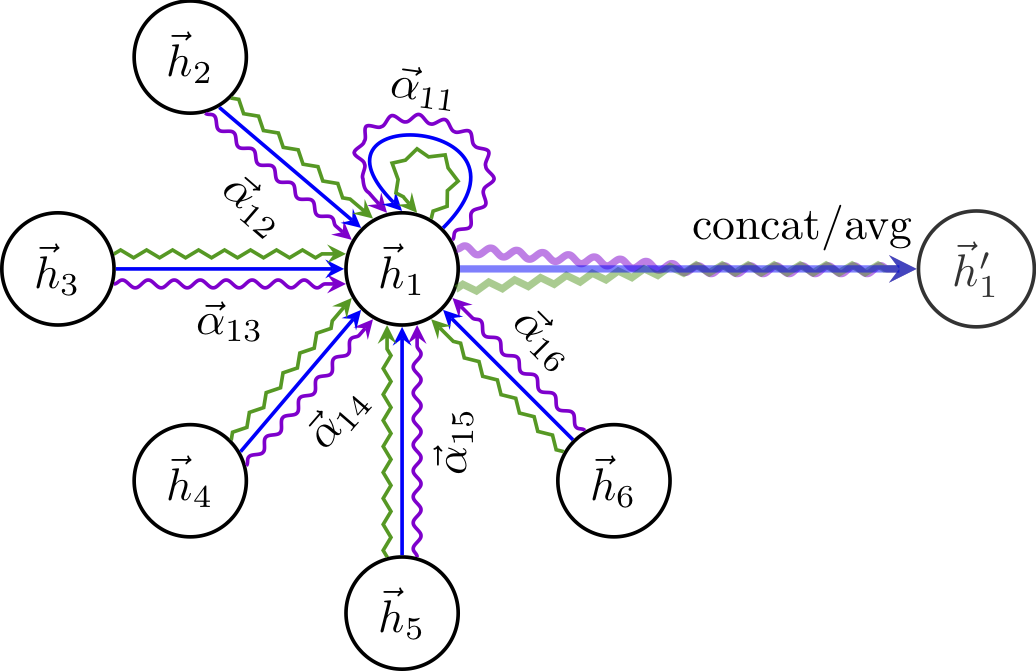
\includegraphics[width=0.5\textwidth]{img/multi_head.png}
    \caption{Multi-head attention with three heads by node $h_1$. \cite{velickovic2018graph}}
    \label{fig:multi-head}
\end{figure}
Allthough this architexture has similarities with prior methods, it solves several issues with its flexibility. We will refer to the original paper for more details but mention two desirable properties that will be important for the subsequent chapters. 

\begin{itemize}[leftmargin=*]
    \item Assigning different importances to nodes of the same neighborhood enables a leap in complexity when compared to graph convolutional networks (GCNs). Furthermore, analyzing the learned attention weights may improve \textbf{explainability} of the model.
    \item Since attention mechanism and feature weight matrix are applied in a shared manner, a trained GAT can be applied to \textbf{inductive} tasks. That is, they can be evaluated on graphs that were completely unseen during training. Many previous approaches depended on upfront access to the whole graph, making them unfeasible for such tasks. 
    \bigskip
\end{itemize}

